%\documentclass[hyperref={pdfpagelabels=false}]{beamer}
\documentclass[aspectratio=1610]{beamer}

%\usetheme{Boadilla}

\usepackage[latin1]{inputenc}
\usepackage{chronology}
\usepackage{mathrsfs}
\usepackage{graphicx}
\usepackage{multicol}
\usepackage{colortbl}
\usepackage{longtable}
\usepackage{diagbox}
\newcolumntype{g}{>{\columncolor{Gray}}r}
\newcolumntype{h}{>{\columncolor{green}}r}
\newcolumntype{y}{>{\columncolor{yellow}}r}
\usepackage{hyperref}

\usepackage{stackengine}
\newcommand\xrowht[2][0]{\addstackgap[.5\dimexpr#2\relax]{\vphantom{#1}}}
\newcommand{\framedhref}[2]{\href{#1}{\fbox{#2}}}


\usepackage{xcolor}
\usepackage{amsmath,amssymb}
\usepackage{comment}
\usepackage{caption}
\usepackage{subcaption}
\usepackage{graphicx}
\usepackage{amssymb} 

\usepackage{xcolor}

\usepackage{bbm}
\usepackage{booktabs}
\newsavebox{\tablebox}
\usepackage{placeins}
\usepackage{dsfont}

\usepackage{tikz}
\newcommand{\ovalframedhref}[2]{%
	\tikz[baseline]{
		\node[anchor=base, draw, ellipse, inner sep=2pt] (link) {\hyperlink{#1}{#2}};
	}%
}

\usetikzlibrary{shapes.geometric}
\usetikzlibrary{shapes,arrows}
\usetikzlibrary{calc}
\usepackage{standalone}
\hypersetup{colorlinks=true,citecolor=gray,linkcolor=blue,urlcolor=blue}
\usepackage{csquotes}
\usepackage{amssymb}
\usepackage{subcaption}
\usepackage{pdfpages}
\usepackage{bbm}
%\usepackage[utf8]{inputenc}
%\usepackage{color, colortbl}
%\definecolor{Gray}{gray}{0.9}
%\definecolor{LightCyan}{rgb}{0.88,1,1}
%\usepackage[first=0,last=9]{lcg}
%\newcommand{\ra}{\rand0.\arabic{rand}}
%\usepackage{standalone}
%\usepackage{beamerthemesplit}
\usepackage{graphicx} 
%\usepackage{threeparttable}
\usepackage{amsmath}
\usepackage{amssymb}
\usepackage{bbm}

\usepackage[scaled]{helvet}
\usepackage[round]{natbib}
\usepackage{chngcntr}
\usepackage{tikz}
\usepackage{systeme}
\usepackage[english]{babel}
\usepackage{pifont}
\usepackage{graphicx}
\usepackage{pgfpages}
\usepackage{csquotes}
\usepackage{ulem}
\usepackage{amsmath}
%\usetheme{Madrid}
\setbeamercovered{transparent}
\setbeamertemplate{theorems}[numbered] \theoremstyle{plain}
\newtheorem{lem}{\underline{Lemme}}[section]
\newtheorem{ppte}{\underline{Propri\'et\'e}}[section]
\newtheorem{algo}{\underline{Algorithmique de construction TOB}}[section]
\newtheorem{propo}{\underline{Proposition}}[section]
\newtheorem{theo}{\underline{Th\'eor$\grave{e}$me}}[section]
\newtheorem{defi}{\underline{D\'efinition}}[section]
\newtheorem{cor}{\underline{Corollaire}}[section]
\newtheorem{rap}{\underline{Rappels}}[section]
\newtheorem{remark}{\underline{Remarque}}[section]
\newtheorem{notation}{\underline{Notation}}[section]
\newtheorem{ex}{Exemple}
\newtheorem{hypothese}{\underline{Hypoth?se}}[section]
\newenvironment{prev}[1][Preuve]{\textbf{#1} }{\ \rule{0.5em}{0.5em}}
\definecolor{my}{rgb}{0.1, 0.9, 0.9}
\definecolor{myt}{rgb}{0.9, 0.5, 0.5}
\newcommand{\ess}{\textrm{ess}\,\sup }
\newcommand{\Conv}{\textrm{Conv\, }}
\newcommand{\Fr}{\textrm{Fr\,}}
\newcommand{\cl}{\textrm{cl\,}}
\newcommand{\grad}{\textrm{grad\,}}
\newcommand{\ch }{\textrm{ch\,}}
\newcommand{\tha }{\textrm{th\,}}
\newcommand{\Argth }{\textrm{Arg\,th\,}}
\newcommand{\sh}{\textrm{sh\,}}
\newcommand{\Argmin}{\textrm{Argmin\,}}
\newcommand{\Argmax}{\textrm{Argmax\,}}
\newcommand{\Argsh}{\textrm{Arg\,sh\,}}
\newcommand{\Log }{\textrm{Log\,}}
\newcommand{\Arccos }{\textrm{Arc\,cos\,}}
\newcommand{\Arcsin }{\textrm{Arc\,sin\,}}
\newcommand{\Arctg }{\textrm{Arc\,tg\,}}
\newcommand{\tg }{\textrm{tg\,}}
\newcommand{\ops }{probl?mes d'optimisation }
\newcommand{\op }{probl?me d'optimisation }
\newcommand{\pr }{probl?me}
\newcommand{\card }{\textrm{card\,}}
\newcommand{\cotg }{\textrm{cotg\,}}
\newcommand{\co }{\textrm{Conv}}
\newcommand{\Arccotg }{\textrm{Arc\,cotg\,}}
\newcommand{\N }{\textrm{$\mathbb{N}$}}
\newcommand{\Z }{\textrm{$\mathbb{Z}$}}
\newcommand{\D }{\textrm{$\mathbb{D}$}}
\newcommand{\T }{\textrm{$\mathbb{T}$}}
\newcommand{\C }{\textrm{$\mathbb{C}$}}
\newcommand{\Q }{\textrm{$\mathbb{Q}$}}
\newcommand{\va }{\textrm{$\varepsilon$}}
\newcommand{\R}{\mathbb{R}}

\usepackage{graphicx} % Allows including images
\usepackage{booktabs} % Allows the use of \toprule, \midrule and \bottomrule in tables
\usepackage{pdfpages}
\usepackage{color}
\usepackage{amsmath}
\usepackage{adjustbox}
\usepackage{rotating}
\usepackage{threeparttable}

\mode<presentation>
{
	\usetheme{default}      % or try Darmstadt, Madrid, Warsaw, ...
	\usecolortheme{default} % or try albatross, beaver, crane, ...
	\usefonttheme{default}  % or try serif, structurebold, ...
	\setbeamertemplate{navigation symbols}{}
	\setbeamertemplate{caption}[numbered]
} 
\usepackage[english]{babel}

\title[]{Capital One Airline Data Challenge.}
\author{by Sossou Simplice Adjisse}
\institute{% Ag. \&  Applied Economics \\ University of Wisconsin-Madison
}
\date{\today}




\begin{document}
	
%	\maketitle
%	\addtocounter{framenumber}{-1}

	\begin{frame}
		\titlepage
	\end{frame}
	
	\begin{frame}
		\tableofcontents
	\end{frame}
	



\section{Context}
\begin{frame}{Context}
	A new airline company is looking to enter the US domestic market and punctuality is a big part of the company's brand image. I am asked to: 
	\begin{enumerate}
		\item find out the 10 busiest round trip routes in terms of a number of round trip flights in the quarter without the canceled flights. 
		\item find out the 10 most profitable round trip routes (without considering the upfront airplane cost) in the quarter and show  profit,  total revenue, total cost, summary values of other key components, and total round trip flights in the quarter for the top 10 most profitable routes without canceled flights.
		\item recommend  5 round trip routes to invest in
		\item calculate the number of round trip flights it will take to breakeven on the upfront airplane cost for each my recommended 5 round trip routes and print key summary components for them
		\item recommend Key Performance Indicators (KPI's) to track in the future to measure the success of the recommended round trip routes. 
		
	\end{enumerate}
\end{frame}

\section{Datasets : Quality, Cleaning, Restrictions, and Limitation}
\begin{frame}{Datasets : Quality, Cleaning, Restrictions, and Limitation}
	\begin{itemize}
		\item Datasets $\Longrightarrow$ flights, tickects, airport\_codes
		\vspace{0.2cm}
		\item All the columns have the intended values
				\vspace{0.2cm}
		\item Some columns have the wrong format $\Longrightarrow$  I converted to right format.
				\vspace{0.2cm}
		\item Outliers in some of the numeric columns $\Longrightarrow$ I kept them
				\vspace{0.2cm}
		\item Numeric columns with missing values $\Longrightarrow$ I replaced them with medians
				\vspace{0.2cm}
		\item Invalid strings (e.g., airport codes) $\Longrightarrow$ I dropped them 
				\vspace{0.2cm}
		\item Duplicates with respect to all the columns $\Longrightarrow$ I dropped them 
				\vspace{0.2cm}
		\item Restrictions $\Longrightarrow$ dropped cancelled flights, non-roundtrips, non-US airports
				\vspace{0.2cm}
        \item Limitation $\Longrightarrow$ lack of information to link tickets to their  flights
	\end{itemize}
\end{frame}

\section{Data: Aggregating and Merging}
\begin{frame}{Data: Aggregating and Merging}
	After cleaning and putting the necessary restrictions on the data:
		\vspace{0.2cm}
	\begin{itemize}
		\item merge the flights and airport codes on ORIGIN and IATA\_CODES as keys, respectively and inner join $\Longrightarrow$ ensured origin of flights are within the US
			\vspace{0.2cm}
		\item merge the flights and airport codes on DESTINATION and IATA\_CODES  as keys respectively an inner join $\Longrightarrow$ ensured destination of flights are within the US
			\vspace{0.2cm}
		\item create ROUTE\_ID for the routes $\Longrightarrow$ routes' unique identifier  in flights dataset
			\vspace{0.2cm}
		\item merge  the tickets and airport codes on DESTINATION and IATA\_CODES as keys respectively and inner join $\Longrightarrow$ ensured destination of tickets are within the US
					\vspace{0.2cm}
		\item create ROUTE\_ID for the routes $\Longrightarrow$ routes' unique identifier  in tickets dataset
			\vspace{0.2cm}
		\item aggregate PASSENGER, ITIN\_FARE , and ROUTRIP at ROUTE\_ID level
			\vspace{0.2cm}
		\item merge back to the previous  combined flights and airport codes on ROUTE\_ID as key and inner join $\Longrightarrow$ final combined data
	\end{itemize}
\end{frame}

\section{Data: Final}
\begin{frame}{Final Data}
	\begin{figure}[htp!]
		\begin{center}
			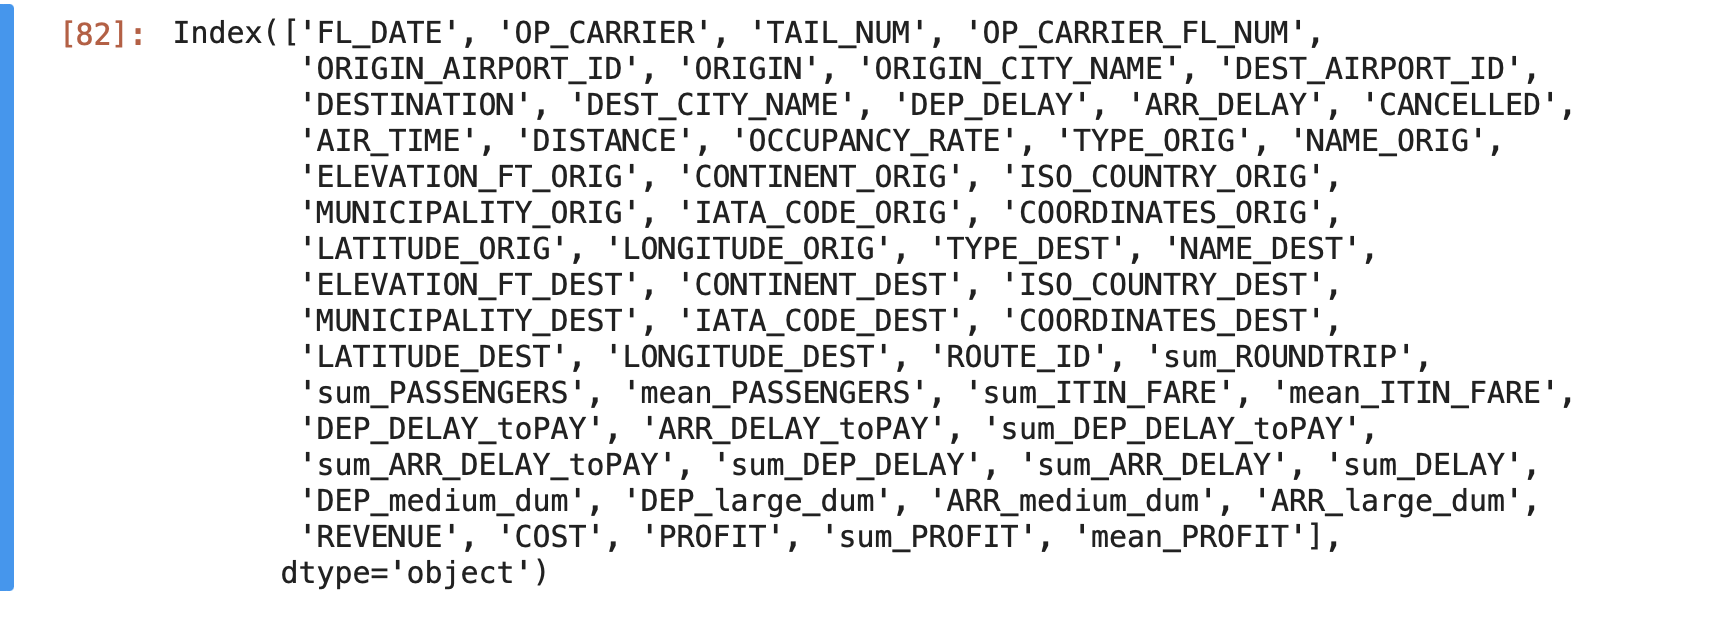
\includegraphics[height=5cm, width= 12cm]{finalData} 
			\caption{ }
			\label{finalData}
		\end{center}
	\end{figure}
\end{frame}

\section{Top 10 Busiest Routes in Terms of Total Round Trip}
\begin{frame}{Top 10 Busiest Routes in Terms of Total Round Trip}
	\begin{figure}[htp!]
		\begin{center}
			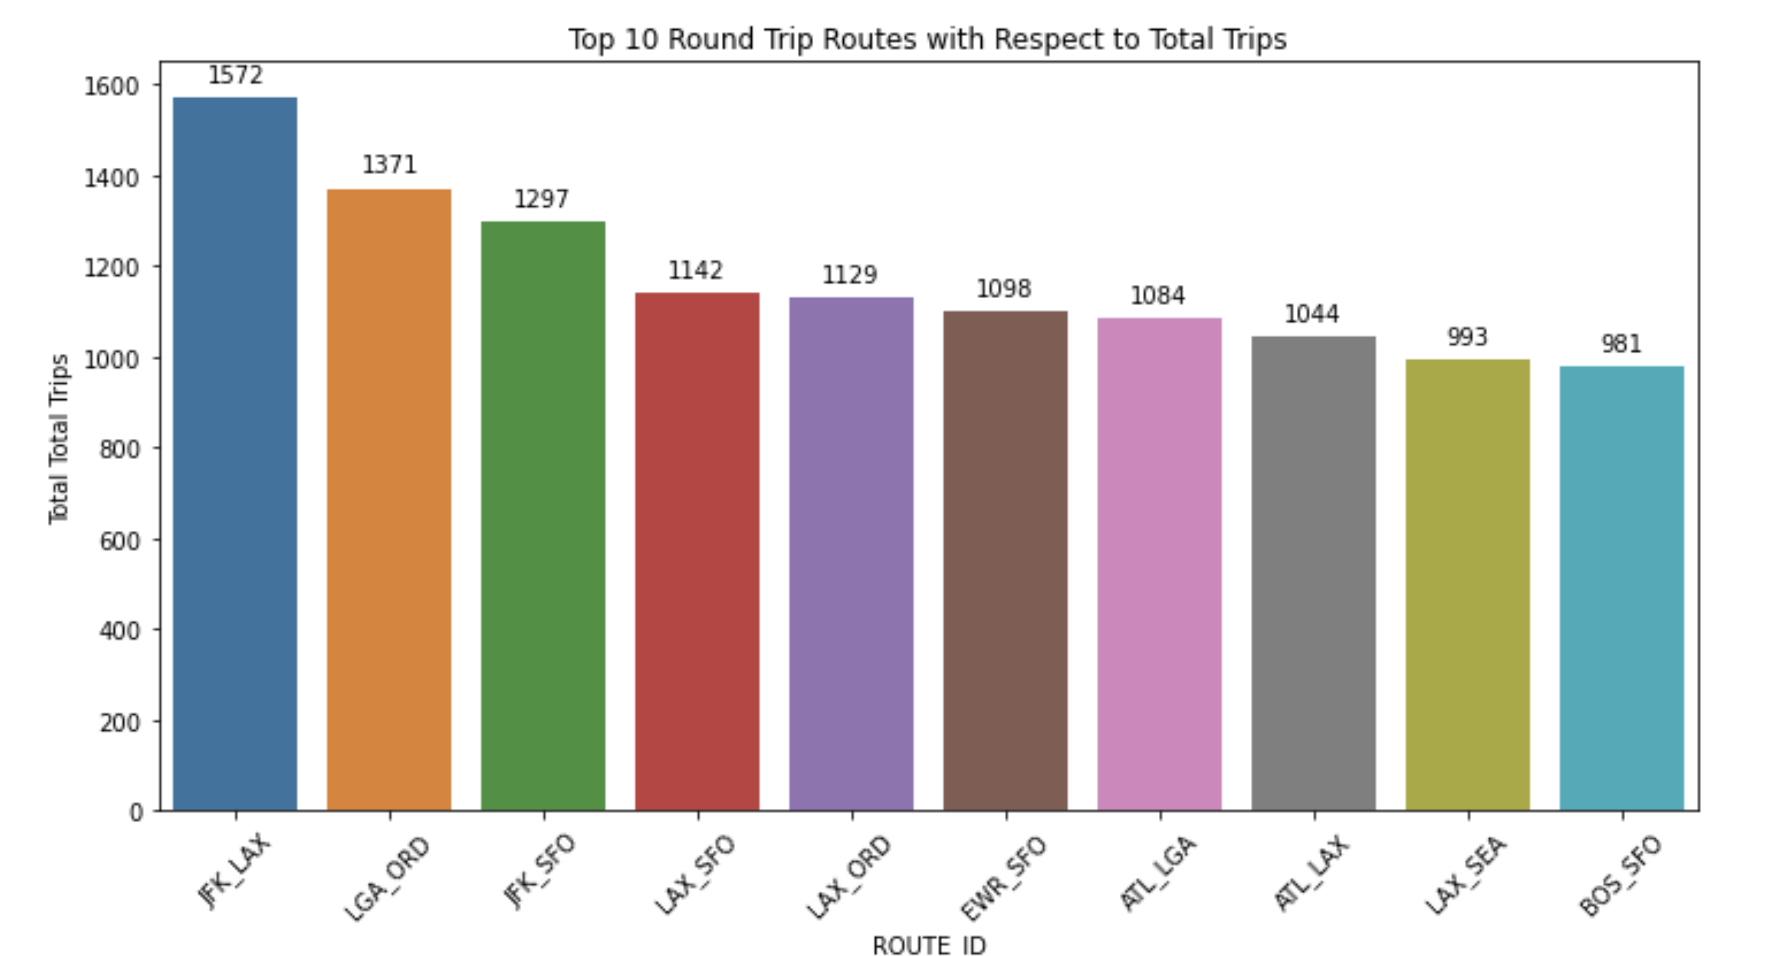
\includegraphics[height=6cm, width= 12cm]{TopBusy} 
			\caption{}
			\label{TopBusy}
		\end{center}
	\end{figure}
\end{frame}

\section{Top 10 Profitable Routes}
\begin{frame}{Top 10 Profitable Routes}
	\begin{figure}[htp!]
		\begin{center}
			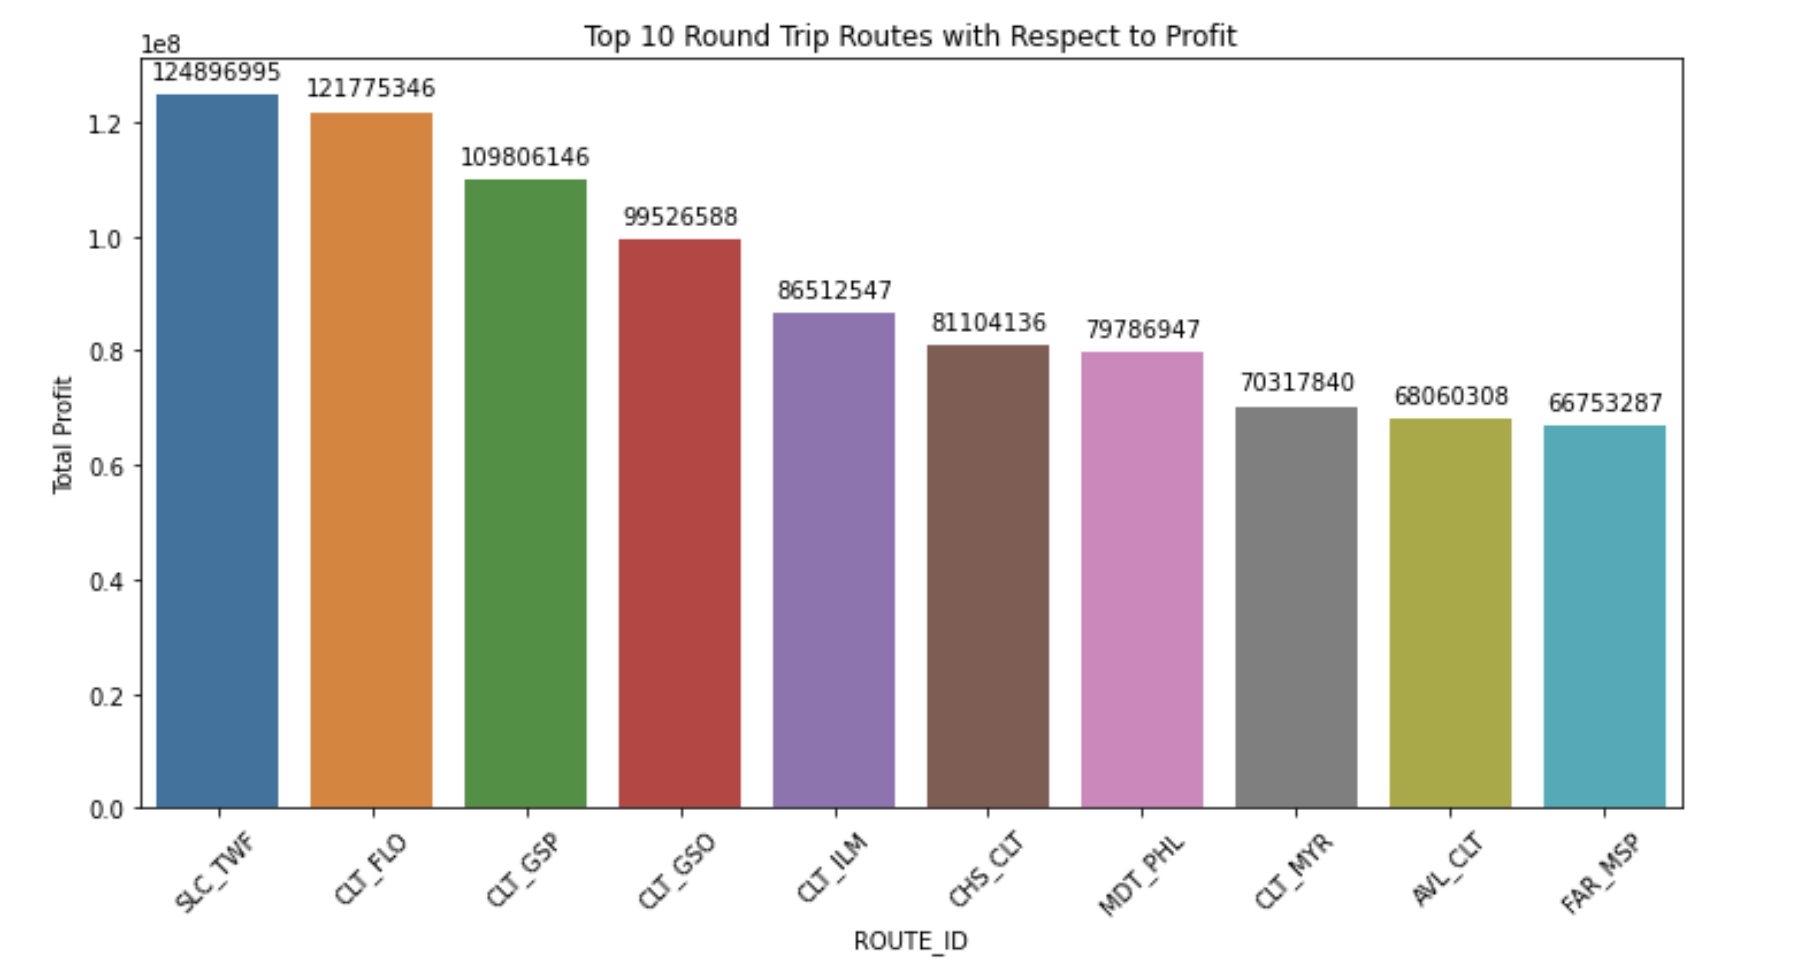
\includegraphics[height=6cm, width= 12cm]{TopProfitable} 
			\caption{}
			\label{TopProfitable}
		\end{center}
	\end{figure}
\end{frame}

\begin{frame}{Top 5 Routes I Recommend the Company Invest in}
	\begin{figure}[htp!]
		\begin{center}
			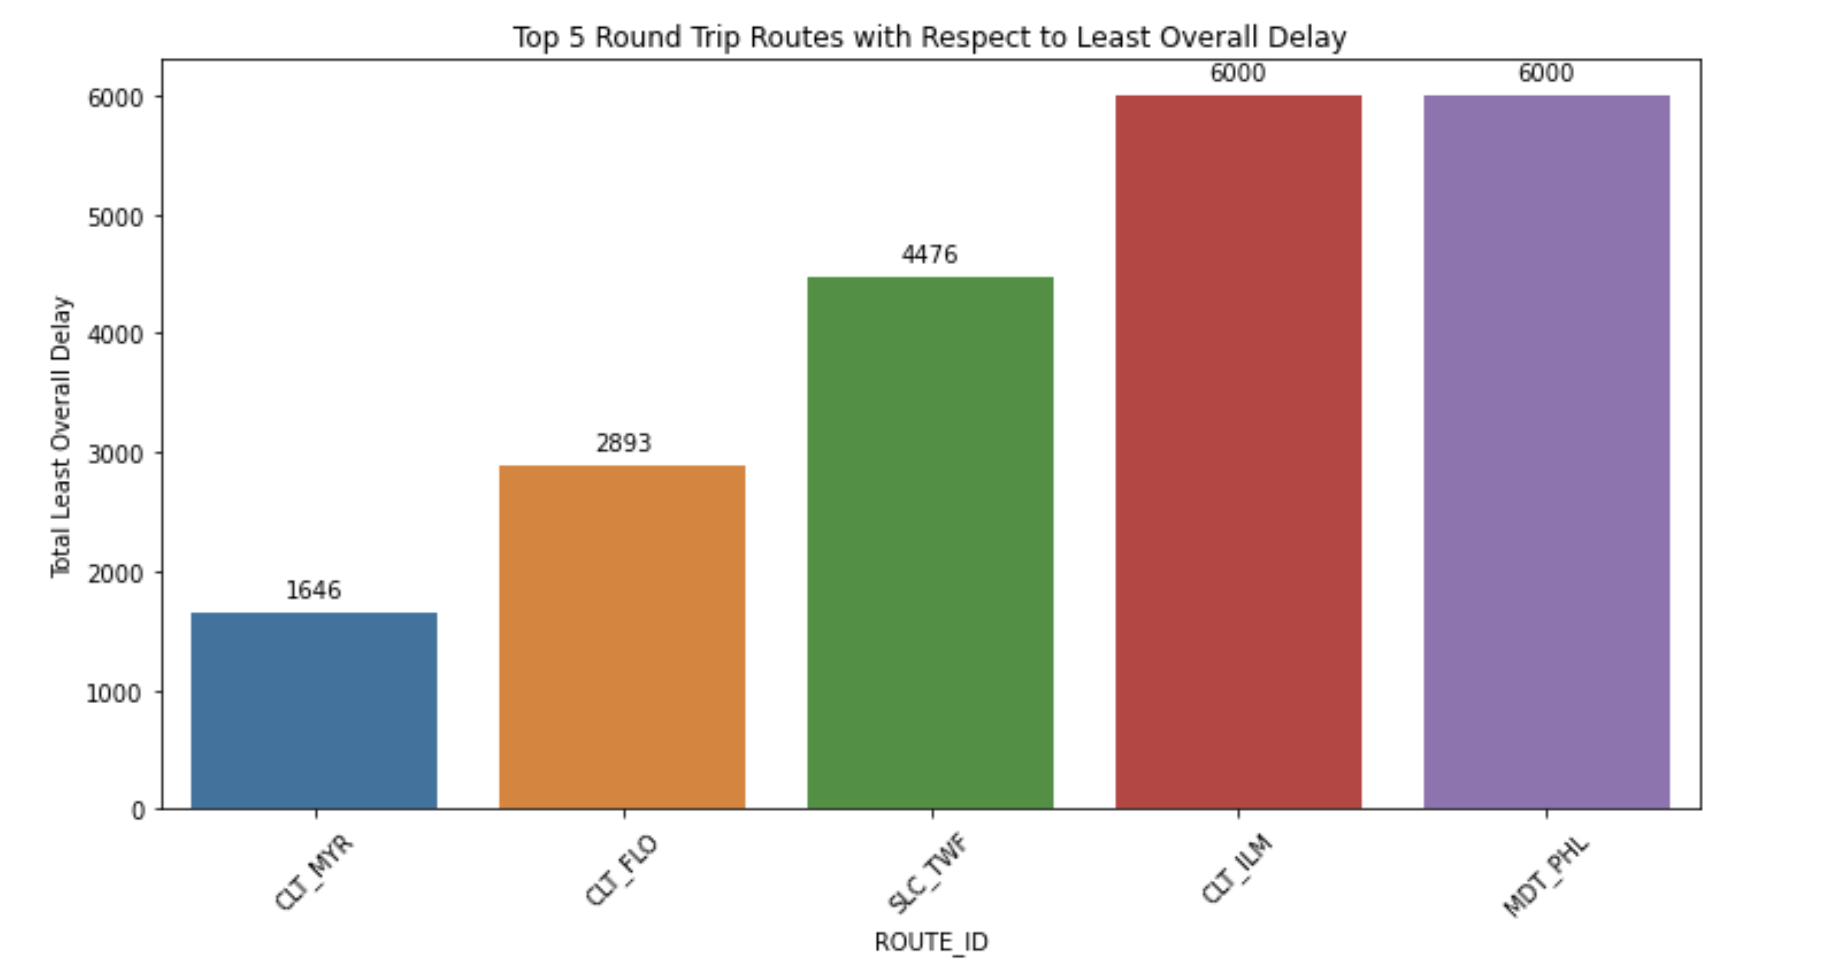
\includegraphics[height=6cm, width= 12cm]{Top5Recom} 
			\caption{}
			\label{Top5Recomended}
		\end{center}
	\end{figure}
\end{frame}

\begin{frame}{Summay Statistics of Key Performane Indicators}
	\begin{figure}[htp!]
		\begin{center}
			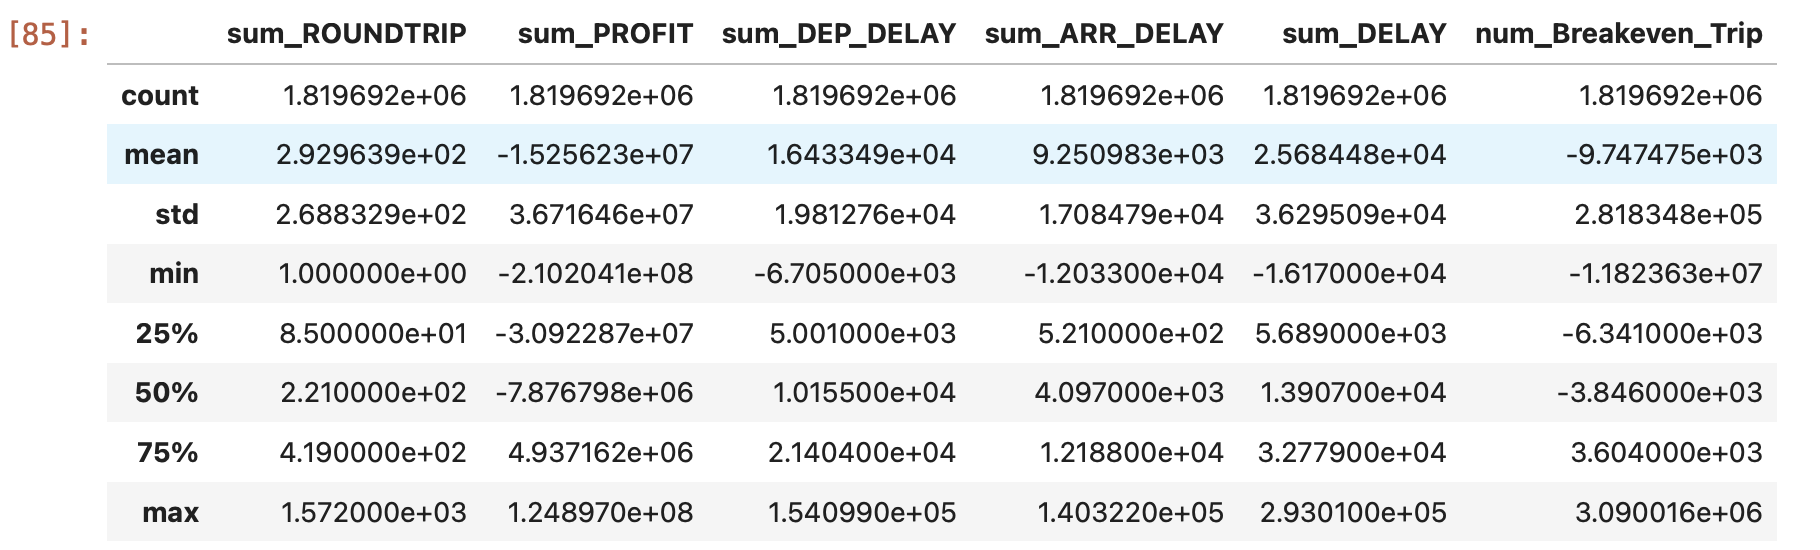
\includegraphics[height=6cm, width= 12cm]{SumStats} 
			\caption{}
			\label{SummaryStats}
		\end{center}
	\end{figure}
\end{frame}

\begin{frame}{Top 10 Leats}
	\begin{figure}[htp!]
		\begin{center}
			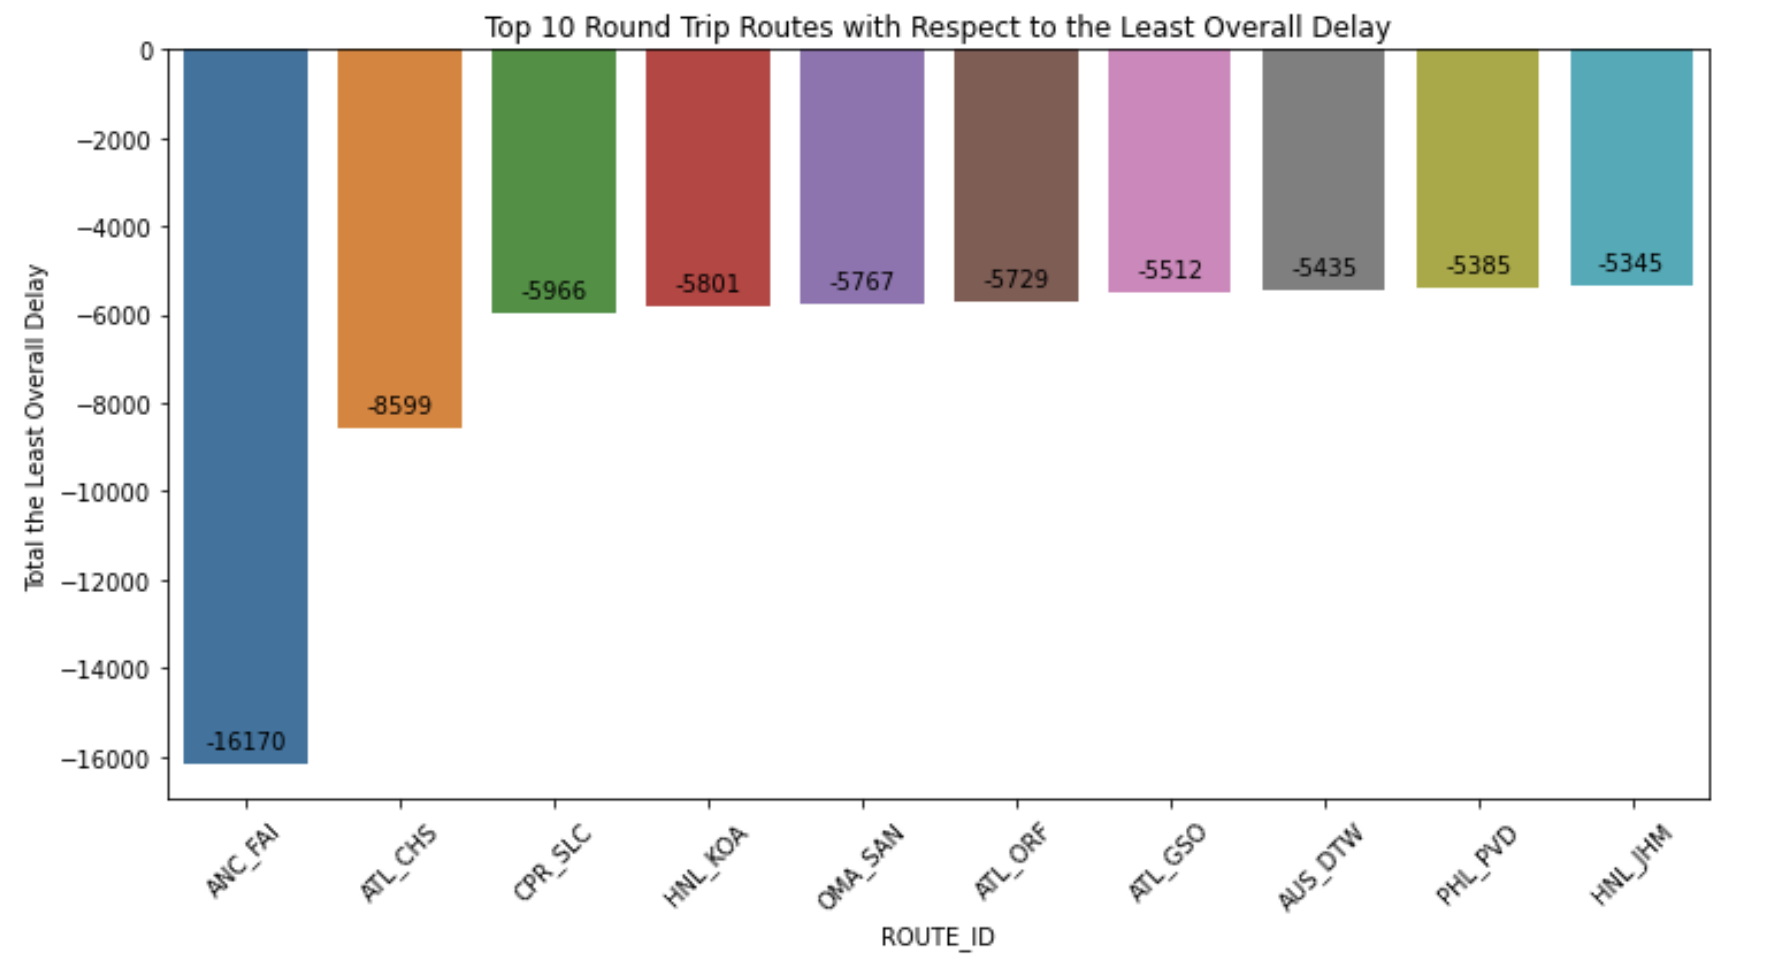
\includegraphics[height=6cm, width= 12cm]{LestDelayed} 
			\caption{}
			\label{LestDelaye}
		\end{center}
	\end{figure}
\end{frame}


\begin{frame}{Top 5 Routes I Recommend the Company Invest in}{They are from the 10 top most profitable routes in Figure \ref{TopProfitable}}
	\begin{figure}[htp!]
		\begin{center}
			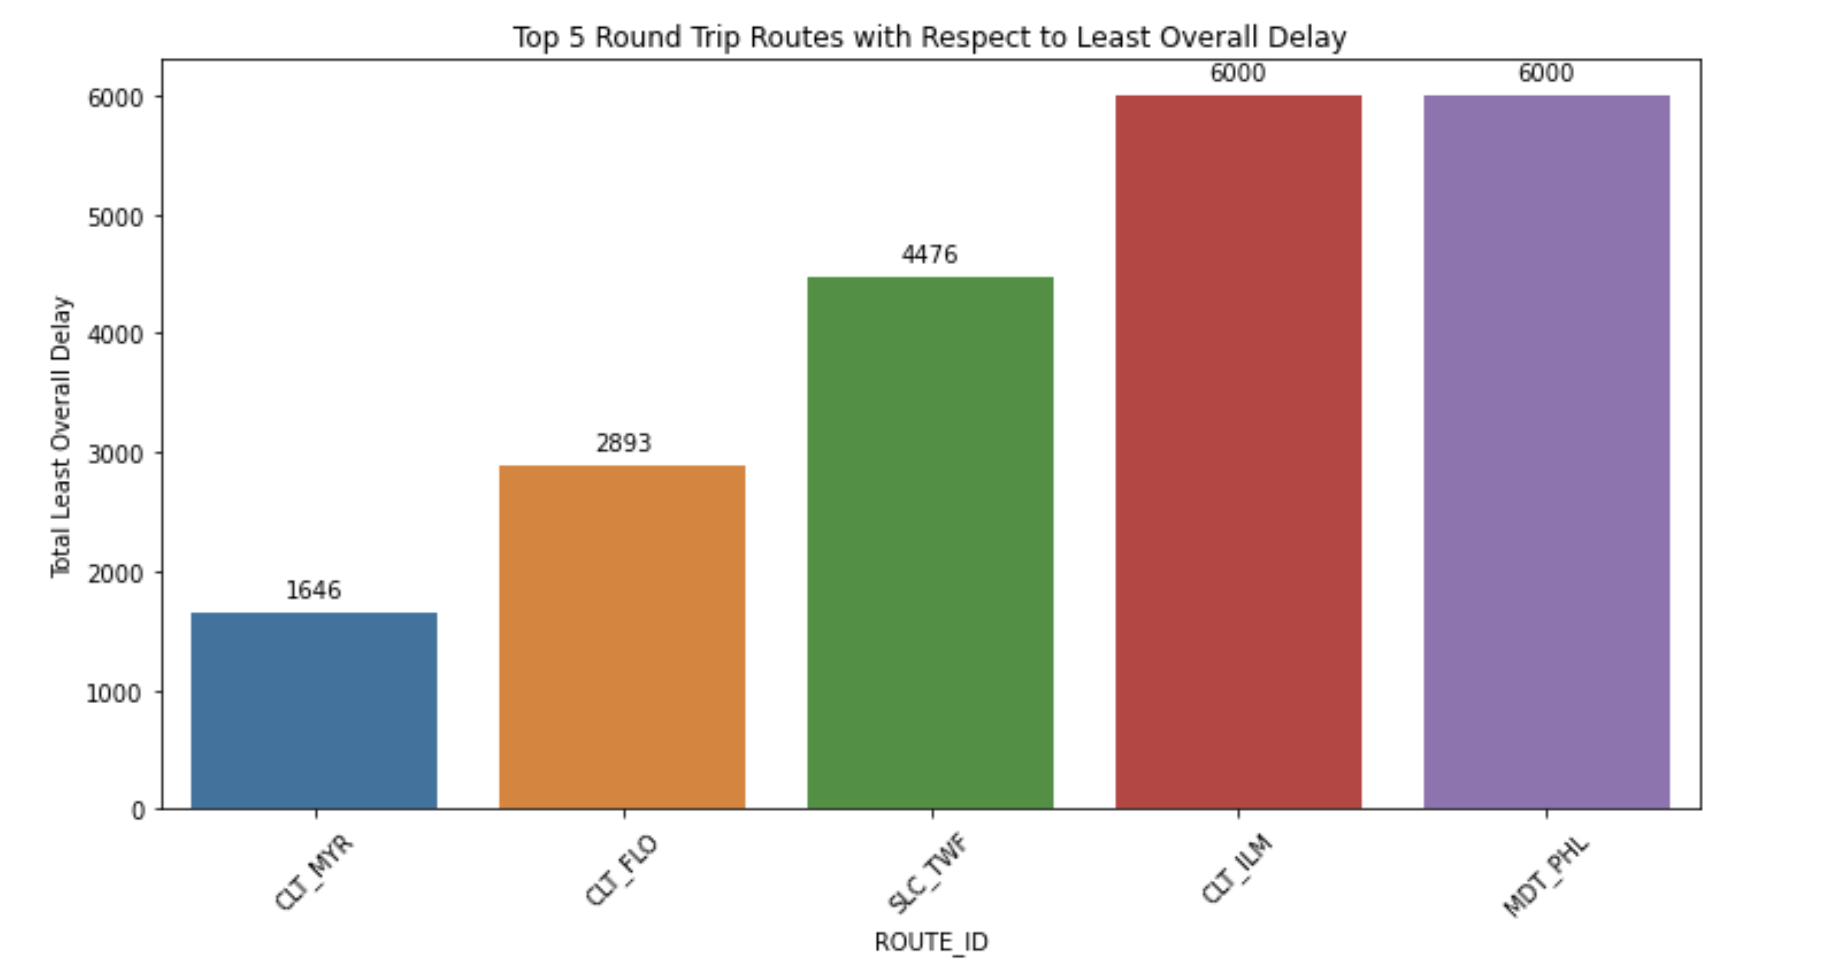
\includegraphics[height=6cm, width= 12cm]{Top5Recom} 
			\caption{}
			\label{Top5Recom}
		\end{center}
	\end{figure}
\end{frame}

\begin{frame}{Key things to Track in the Future}
	\begin{itemize}
		\item Competitions, entrance cost, opportunity cost, comparative advantages
		\item Most profitable routes which have the least delay
		\item Delay metrics:
		\begin{itemize}
			\item departure delay
			\item arrival delay
			\item Overall delay
		\end{itemize}
	\end{itemize}
\end{frame}

\end{document}